\chapter*{Dodatak: Prikaz aktivnosti grupe}
		\addcontentsline{toc}{chapter}{Dodatak: Prikaz aktivnosti grupe}
		
		\section*{Dnevnik sastajanja}
		
		%\textbf{\textit{Kontinuirano osvježavanje}}\\
		
		 %\textit{U ovom dijelu potrebno je redovito osvježavati dnevnik sastajanja prema predlošku.}
		
		\begin{packed_enum}
			
			\item  sastanak
			
			\item[] \begin{packed_item}
				\item Datum: 18.listopada 2023.
				\item Prisustvovali: J. Balatinec, I. Cvrk, V. Đurić, S. Kiš, A. Kućar, M. Štambuk, I. Žagar
				\item Teme sastanka:
				\begin{packed_item}
					\item  Inicijalni sastanak
					\item  Diskusija o početku rada
					\item  Upoznavanje sa zadatkom
				\end{packed_item}
			\end{packed_item}
			
			\item  sastanak
			
			\item[] \begin{packed_item}
				\item Datum: 25.listopada 2023.
				\item Prisustvovali: J. Balatinec, I. Cvrk, V. Đurić, S. Kiš, A. Kućar, M. Štambuk, I. Žagar
				\item Teme sastanka:
				\begin{packed_item}
					\item  Diskusija o radu s alatima za pisanje dokumentacije
					\item  Diskusija o stavljanju i preuzimanju na/s GitHub-a
					\item  Podjela rada za do sljedećeg sastanka
				\end{packed_item}
			\end{packed_item}
			
			\item  sastanak
			
			\item[] \begin{packed_item}
				\item Datum: 15.studenog 2023.
				\item Prisustvovali: J. Balatinec, V. Đurić, A. Kućar, I. Žagar
				\item Teme sastanka:
				\begin{packed_item}
					\item  Diskusija s demonstratoricom oko dosadašnjeg napretka na projektu
					\item  Diskusija o daljnjim koracima razvoja i zadacima na projektu
				\end{packed_item}
			\end{packed_item}
			
			\item  sastanak
			
			\item[] \begin{packed_item}
				\item Datum: 16.studenog 2023.
				\item Prisustvovali: J. Balatinec, I. Cvrk, V. Đurić, S. Kiš, A. Kućar
				\item Teme sastanka:
				\begin{packed_item}
					\item  Diskusija o svemu što je napravljeno na projektu
					\item  Dovršavanje implementacije i ispravak dokumentacije
					\item  Diskusija o daljnjem radu na projektu
				\end{packed_item}
			\end{packed_item}
			
			\item  sastanak
			
			\item[] \begin{packed_item}
				\item Datum: 13.prosinca 2023.
				\item Prisustvovali: V. Đurić
				\item Teme sastanka:
				\begin{packed_item}
					\item  Diskusija s demonstratoricom o prvom kolokviranju projekta
					\item  Diskusija s demonstratoricom o dijagramima obrazaca uporabe
				\end{packed_item}
			\end{packed_item}
			
			%
			
		\end{packed_enum}
		
		\eject
		\section*{Tablica aktivnosti}
		
			%\textbf{\textit{Kontinuirano osvježavanje}}\\
			
%			 \textit{Napomena: Doprinose u aktivnostima treba navesti u satima po članovima grupe po aktivnosti.}

			\begin{longtblr}[
					label=none,
				]{
					vlines,hlines,
					width = \textwidth,
					colspec={X[7, l]X[1, c]X[1, c]X[1, c]X[1, c]X[1, c]X[1, c]X[1, c]}, 
					vline{1} = {1}{text=\clap{}},
					hline{1} = {1}{text=\clap{}},
					rowhead = 1,
				} 
			
				\SetCell[c=1]{c}{} & \SetCell[c=1]{c}{\rotatebox{90}{\textbf{Vinko Đurić}}} & \SetCell[c=1]{c}{\rotatebox{90}{\textbf{Josip Balatinec}}} &	\SetCell[c=1]{c}{\rotatebox{90}{\textbf{Ivan Cvrk }}} & \SetCell[c=1]{c}{\rotatebox{90}{\textbf{Stella Kiš }}} &	\SetCell[c=1]{c}{\rotatebox{90}{\textbf{Anđelko Kućar }}} & \SetCell[c=1]{c}{\rotatebox{90}{\textbf{Marina Štambuk }}} &	\SetCell[c=1]{c}{\rotatebox{90}{\textbf{Ivan Žagar }}} \\  
				Upravljanje projektom 				& 17 &  &  &  &  &  & \\ 
				Opis projektnog zadatka 			& 1 &  &  &  & 1 &  & 6 \\ 
				
				Funkcionalni zahtjevi       		& 1 &  &  & 1 &  &  &  \\ 
				Opis pojedinih obrazaca 			& 7 &  &  & 3 &  & 2 &  \\ 
				Dijagram obrazaca 					& 9 &  &  & 1 &  &  &  \\ 
				Sekvencijski dijagrami 				&  & 6 &  &  &  &  &  \\ 
				Opis ostalih zahtjeva 				& 1 &  &  &  &  &  &  \\ 

				Arhitektura i dizajn sustava	 	& 2 &  &  &  &  &  &  \\ 
				Baza podataka						& 6 &  &  &  &  &  &   \\ 
				Dijagram razreda 					& 8 &  &  &  &  &  &   \\ 
				Dijagram stanja						& 6 &  &  &  &  &  &  \\ 
				Dijagram aktivnosti 				& 5 &  &  &  &  &  &  \\ 
				Dijagram komponenti					& 3 &  &  &  &  &  &  \\ 
				Korištene tehnologije i alati 		& 2 &  &  &  &  &  &  \\ 
				Ispitivanje programskog rješenja 	& 1 &  &  &  &  &  & 12 \\ 
				Dijagram razmještaja				& 1 &  &  &  &  &  &  \\ 
				Upute za puštanje u pogon 			& 1 &  & 1 &  &  &  &  \\  
				Dnevnik sastajanja 					& 1 &  &  &  &  &  &  \\ 
				Zaključak i budući rad 				& 1 &  &  &  &  &  &  \\  
				Popis literature 					& 1 &  &  &  &  &  &  \\  
				&  &  &  &  &  &  &  \\ \hline 
				\textit{Frontend} 					&  &  & 50 & 15 &  &  & 29 \\  
				\textit{Backend} 		 			&  & 30 & 25 &  & 99 &  & \\ 
				\textit{Dizajn}						&  &  &  & 4 &  &  &  \\ 
			\end{longtblr}
					
					
		\eject
		\section*{Dijagrami pregleda promjena}
		
		%\textbf{\textit{dio 2. revizije}}\\
		
		%\textit{Prenijeti dijagram pregleda promjena nad datotekama projekta. Potrebno je na kraju projekta generirane grafove s gitlaba prenijeti u ovo poglavlje dokumentacije. Dijagrami za vlastiti projekt se mogu preuzeti s gitlab.com stranice, u izborniku Repository, pritiskom na stavku Contributors.}
		
		
		\begin{figure}[H]
			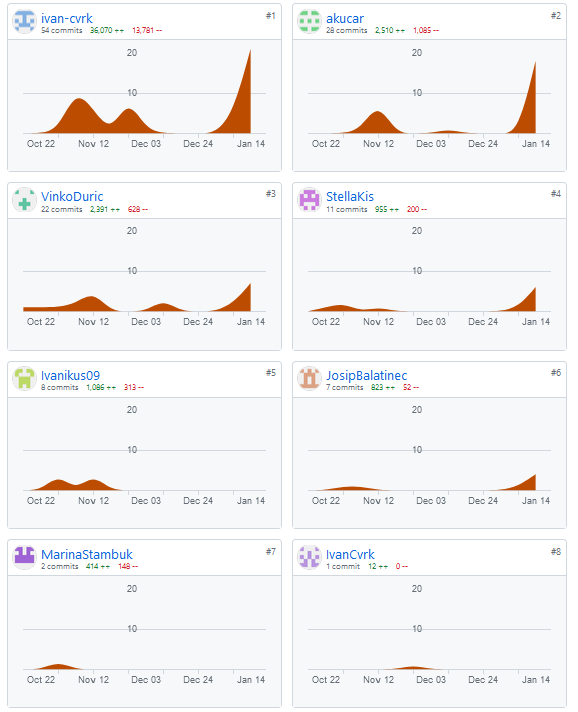
\includegraphics[width=\textwidth]{slike/github3.PNG}
			\caption{GitHub - commitovi po članovima projektnog tima}
			\label{fig:github1}
		\end{figure}
		
		\begin{figure}[H]
			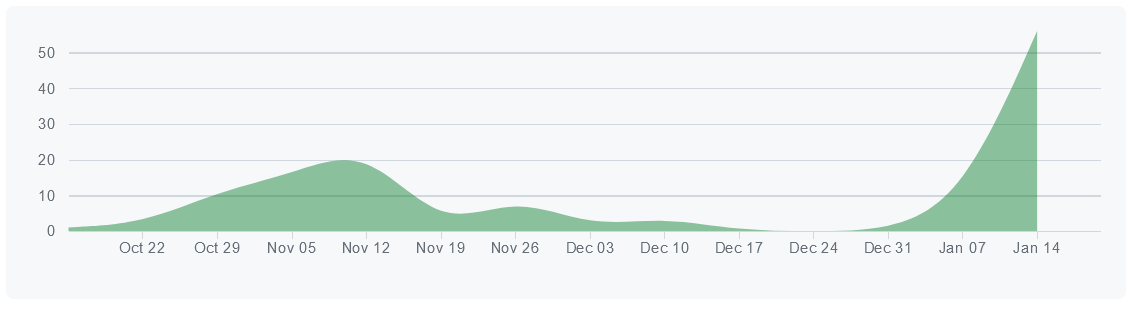
\includegraphics[width=\textwidth]{slike/github4.PNG}
			\caption{GitHub - ukupni commitovi kroz vrijeme}
			\label{fig:github2}
		\end{figure}
		
	